\documentclass[twoside]{article}
\usepackage{aistats2016}
\usepackage{hyperref}
\usepackage{amsmath, amssymb, amsthm, graphicx, algorithm}
\usepackage{algpseudocode}
\usepackage{caption}
\usepackage{subcaption}
\usepackage{blkarray}
\usepackage{xcolor}
\usepackage[all,cmtip]{xy}
\usepackage{caption}
%\usepackage[accepted]{aistats2016}

% If your paper is accepted, change the options for the package
% aistats2016 as follows:
%
%\usepackage[accepted]{aistats2016}
%
% This option will print headings for the title of your paper and
% headings for the authors names, plus a copyright note at the end of
% the first column of the first page.

\newcommand{\A}{\mathcal{A}}
\newcommand{\C}{\mathcal{C}}
\newcommand{\D}{\mathcal{D}}
\newcommand{\G}{\mathcal{G}}
\newcommand{\B}{\mathcal{B}}
\newcommand{\E}{\mathcal{E}}
\newcommand{\cS}{\mathcal{S}}
\newcommand{\U}{\mathcal{U}}
\newcommand{\cL}{\mathcal{L}}
\newcommand{\N}{\mathcal{N}}
\newcommand{\cO}{\mathcal{O}}
\newcommand{\M}{\mathcal{M}}
\newcommand{\bN}{\mathbb{N}}
\newcommand{\bQ}{\mathbb{Q}}
\newcommand{\Exp}{\mathbb{E}}
\newcommand{\bC}{\mathbb{C}}
\newcommand{\bR}{\mathbb{R}}
\newcommand{\bZ}{\mathbb{Z}}
\newcommand{\bK}{\mathbb{K}}
\newcommand{\bF}{\mathbb{F}}

\newcommand{\fF}{\mathbf{F}}
\newcommand{\fA}{\mathbf{A}}
\newcommand{\Grp}{\mathbf{Grp}}
\newcommand{\Set}{\mathbf{Set}}
\newcommand{\Mor}{\mathrm{Mor}}
\newcommand{\Aut}{\mathrm{Aut}}
\newcommand{\Gal}{\mathrm{Gal}}
\newcommand{\Char}{\mathrm{char}}
\newcommand{\SL}{\mathrm{SL}}
\newcommand{\GL}{\mathrm{GL}}
\newcommand{\Span}{\mathrm{span}}
\newcommand{\Hom}{\mathrm{Hom}}
\newcommand{\Ext}{\mathrm{Ext}}
\newcommand{\im}{\mathrm{im}}
\newcommand{\col}{\mathrm{col}}
\newcommand{\argmax}{\mathrm{argmax}}
\newcommand{\cone}{\mathrm{cone}}
\newcommand{\rank}{\mathrm{rank}}
\newcommand{\RP}{\mathbb{R}\mathrm{P}}
\newcommand{\tr}{\mathrm{tr}}

\newcommand{\df}{\overset{\text{def}}{=}}
%\newcommand{\deg}{\mathrm{deg}}

\newcommand{\vx}{\mathbf{x}}
\newcommand{\vy}{\mathbf{y}}
\newcommand{\vu}{\mathbf{u}}
\newcommand{\vv}{\mathbf{v}}
\newcommand{\va}{\mathbf{a}}
\newcommand{\vb}{\mathbf{b}}
\newcommand{\vc}{\mathbf{c}}
\newcommand{\vd}{\mathbf{d}}
\newcommand{\vg}{\mathbf{g}}
\newcommand{\vk}{\mathbf{k}}
\newcommand{\vw}{\mathbf{w}}
\newcommand{\vz}{\mathbf{z}}
\newcommand{\vp}{\mathbf{p}}
\newcommand{\vq}{\mathbf{q}}
\newcommand{\vS}{\mathbf{S}}
\newcommand{\vf}{\mathbf{f}}
\newcommand{\bo}{\mathbf{1}}
\newcommand{\bz}{\mathbf{0}}
\newcommand{\id}{\mathrm{id}}

\theoremstyle{theorem}
\newtheorem{thm}{Theorem}

\theoremstyle{theorem}
\newtheorem{prop}{Proposition}
\theoremstyle{theorem}
\newtheorem{cor}{Corollary}

\theoremstyle{lemma}
\newtheorem{lemma}{Lemma}

\theoremstyle{definition}
\newtheorem{defn}{Definition}

\theoremstyle{example}
\newtheorem{ex}{Example}

\newcommand\undermat[2]{%
  \makebox[0pt][l]{$\smash{\underbrace{\phantom{%
    \begin{matrix}#2\end{matrix}}}_{\text{$#1$}}}$}#2}
    
\newcommand\overmat[2]{%
  \makebox[0pt][l]{$\smash{\color{black}\overbrace{\phantom{%
    \begin{matrix}#2\end{matrix}}}^{\text{\color{black}#1}}}$}#2}


\begin{document}
\input xy
\xyoption{all}
\xyoption{arc}
\makeatletter
\def\BState{\State\hskip-\ALG@thistlm}
\makeatother
% If your paper is accepted and the title of your paper is very long,
% the style will print as headings an error message. Use the following
% command to supply a shorter title of your paper so that it can be
% used as headings.
%
%\runningtitle{I use this title instead because the last one was very long}

% If your paper is accepted and the number of authors is large, the
% style will print as headings an error message. Use the following
% command to supply a shorter version of the authors names so that
% they can be used as headings (for example, use only the surnames)
%
%\runningauthor{Surname 1, Surname 2, Surname 3, ...., Surname n}

\twocolumn[

\aistatstitle{Analyzing Boston 311 Responses with Gaussian Mixture Models}

\aistatsauthor{ Jane Huang \And Isadora Nun \And Weiwei Pan \And Francisco Rivera}

\aistatsaddress{ Harvard University \And Harvard University \And Harvard University \And Harvard University} ]

\begin{abstract}
Fill in later.
We approximate the distribution of the response times, longitude, and latitude of 311 requests as a three-component Gaussian mixture model. 
\end{abstract}

\section{Introduction}

In Boston, thousands of requests are made each week to city non-emergency services to address issues such as graffiti, potholes, and broken traffic signals \cite{walshpressrelease}. Requests made to non-emergency services fall under the umbrella of Boston 311.\footnote{When city non-emergency services was rebranded recently as Boston 311, the Citizens Connect App was renamed BOS:311. We refer to the app as Citizens Connect throughout for continuity.} Ensuring that requests are fulfilled in a timely manner and that services are accessible to all segments of the population is essential for maintaining the safety and well-being of city residents. 

Traditionally, requests for city non-emergency services have been made through phone calls, but after smartphone technology became increasingly common, the Citizens Connect app was introduced in 2009 to allow Boston residents to report problems to 311 through a mobile phone interface \cite{newurbanmechanics}. The app developers state their motivation as: ``Residents report public issues directly from their smart phones into the City's work order management system so that it gets immediately to the right person in City Hall to fix the problem...We were interested in seeing if we could engage more or different residents" \cite{newurbanmechanics}.  

To assess the extent to which the 311 app may facilitate more efficient responses to populations not as well-served through the traditional mode of contacting non-emergency services, we seek to model and compare the joint distribution of response times and locations for 311 requests made via constituent calls and those made via the mobile phone app. [WHICH FIGURES DO WE WANT TO SHOW HERE?] Because we are interested in identifying whether there are hidden sub-populations of requests that are distinguishable by the observed locations and response times, we use Gaussian mixture models to approximate the distributions. 

\section{Data}
Records of Boston's 311 service requests were obtained from \url{https://data.cityofboston.gov/City-Services/311-Service-Requests/awu8-dc52Opens in new window}. We first selected all closed complaints that had been opened in 2015 through constituent calls or the Citizens Connect App. The descriptors extracted for the data included the times that the complaints were opened and closed by the city (reported to the nearest second) and the longitude and latitude of the source of the complaint. A new variable, response time, was defined as the difference between the reported closing and opening times of a 311 complaint. Because the numerical scale of response times is much larger than those of longitude and latitude, the values for each variable were rescaled to have zero mean and unit variance. (The mean response time is 13.2 days with standard deviation 29.1 days. The mean latitude is 42.326 with standard deviation 0.034. The mean longitude is -71.083 with standard deviation 0.035). The data were subsequently split apart into two sets based on whether they originated from constituent calls or Citizens Connect. 

Because the dataset is very large, a randomly selected subsample was used for the analysis to reduce computational expense. For the expectation maximization estimates, the data were downsampled to provide $\sim20,000$ points each for constituent call and Citizens Connect App analysis. For Gibbs sampling, the data were downsampled to provide $\sim10,000$ points for each group. 
\section{Methods}
\subsection{Bayesian Gaussian Mixture Models}

Each 311 request is described by a three-dimensional vector consisting of $x_n$ = (response time, longitude, latitude). We model the distribution of these datapoints as a mixture of $K$ Gaussian components with means $\mu = \{\mu_k :  1\leq k\leq K\}$ and covariance matrices $\Sigma = \{\Sigma_k :  1\leq k\leq K\}$. The mixture coefficients for the model (i.e., the fraction of the population belonging to each component) is represented by $\pi$, a vector with $K$ elements.  

The forms of the equations describing Gaussian mixture models and the conditional distributions are adopted from \cite{Gelman, Jones}.

Since the component membership is not known, we specify the component membership indicators as $\mathbf{Z} = (z_1, \ldots, z_N)$. Each indicator for datapoint $x_n$ is a $K$-element vector $z_n$, defined such that \begin{align}
z_{nk} = \begin{cases}
1, & x_n\text{ belongs to the $k$-th component}\\
0, & \text{otherwise}. 
\end{cases}
\end{align}
Hence, the likelihood of the observations is 
\begin{align}
L(\mathbf{X}) = \prod_{n=1}^N\prod_{k=1}^K \N(x_n| \mu_k, \Sigma_k)^{z_{nk}}.
\end{align}
The prior for $\pi$ is a Dirichlet distribution. For $\Sigma$, we use an inverse-Wishart prior, which is conjugate to the multivariate normal distribution and ensures the selection of a positive-definite matrix. The hyperparameters for the inverse-Wishart prior are the scale matrix $S_0$ and the degrees of freedom $\nu_0$.  These priors can be set to be weakly informative, which is useful because it is difficult to assess \textit{a priori} what the components in the 311 data are. In addition, these priors allow closed forms of the conditional distributions to be used in Gibbs sampling to explore the posterior distribution. 

To summarize, our model is described by the following: 
\begin{align}
\pi &\sim Dir(\alpha_0)\\
\Sigma_k &\sim \mathrm{invWish}(S_0, \nu_0)\\
\mu_k | \Sigma_k &\sim \N(m_0, V_0)\\
z_n | \pi &\sim \prod_{k=1}^K \pi_k^{z_{nk}}\\
x_n | \mathbf{Z}, \mu, \Sigma &\sim \prod_{k=1}^K \N(\mu_k, \Sigma_k)^{z_{nk}}
\end{align}


\begin{figure}
\begin{center}
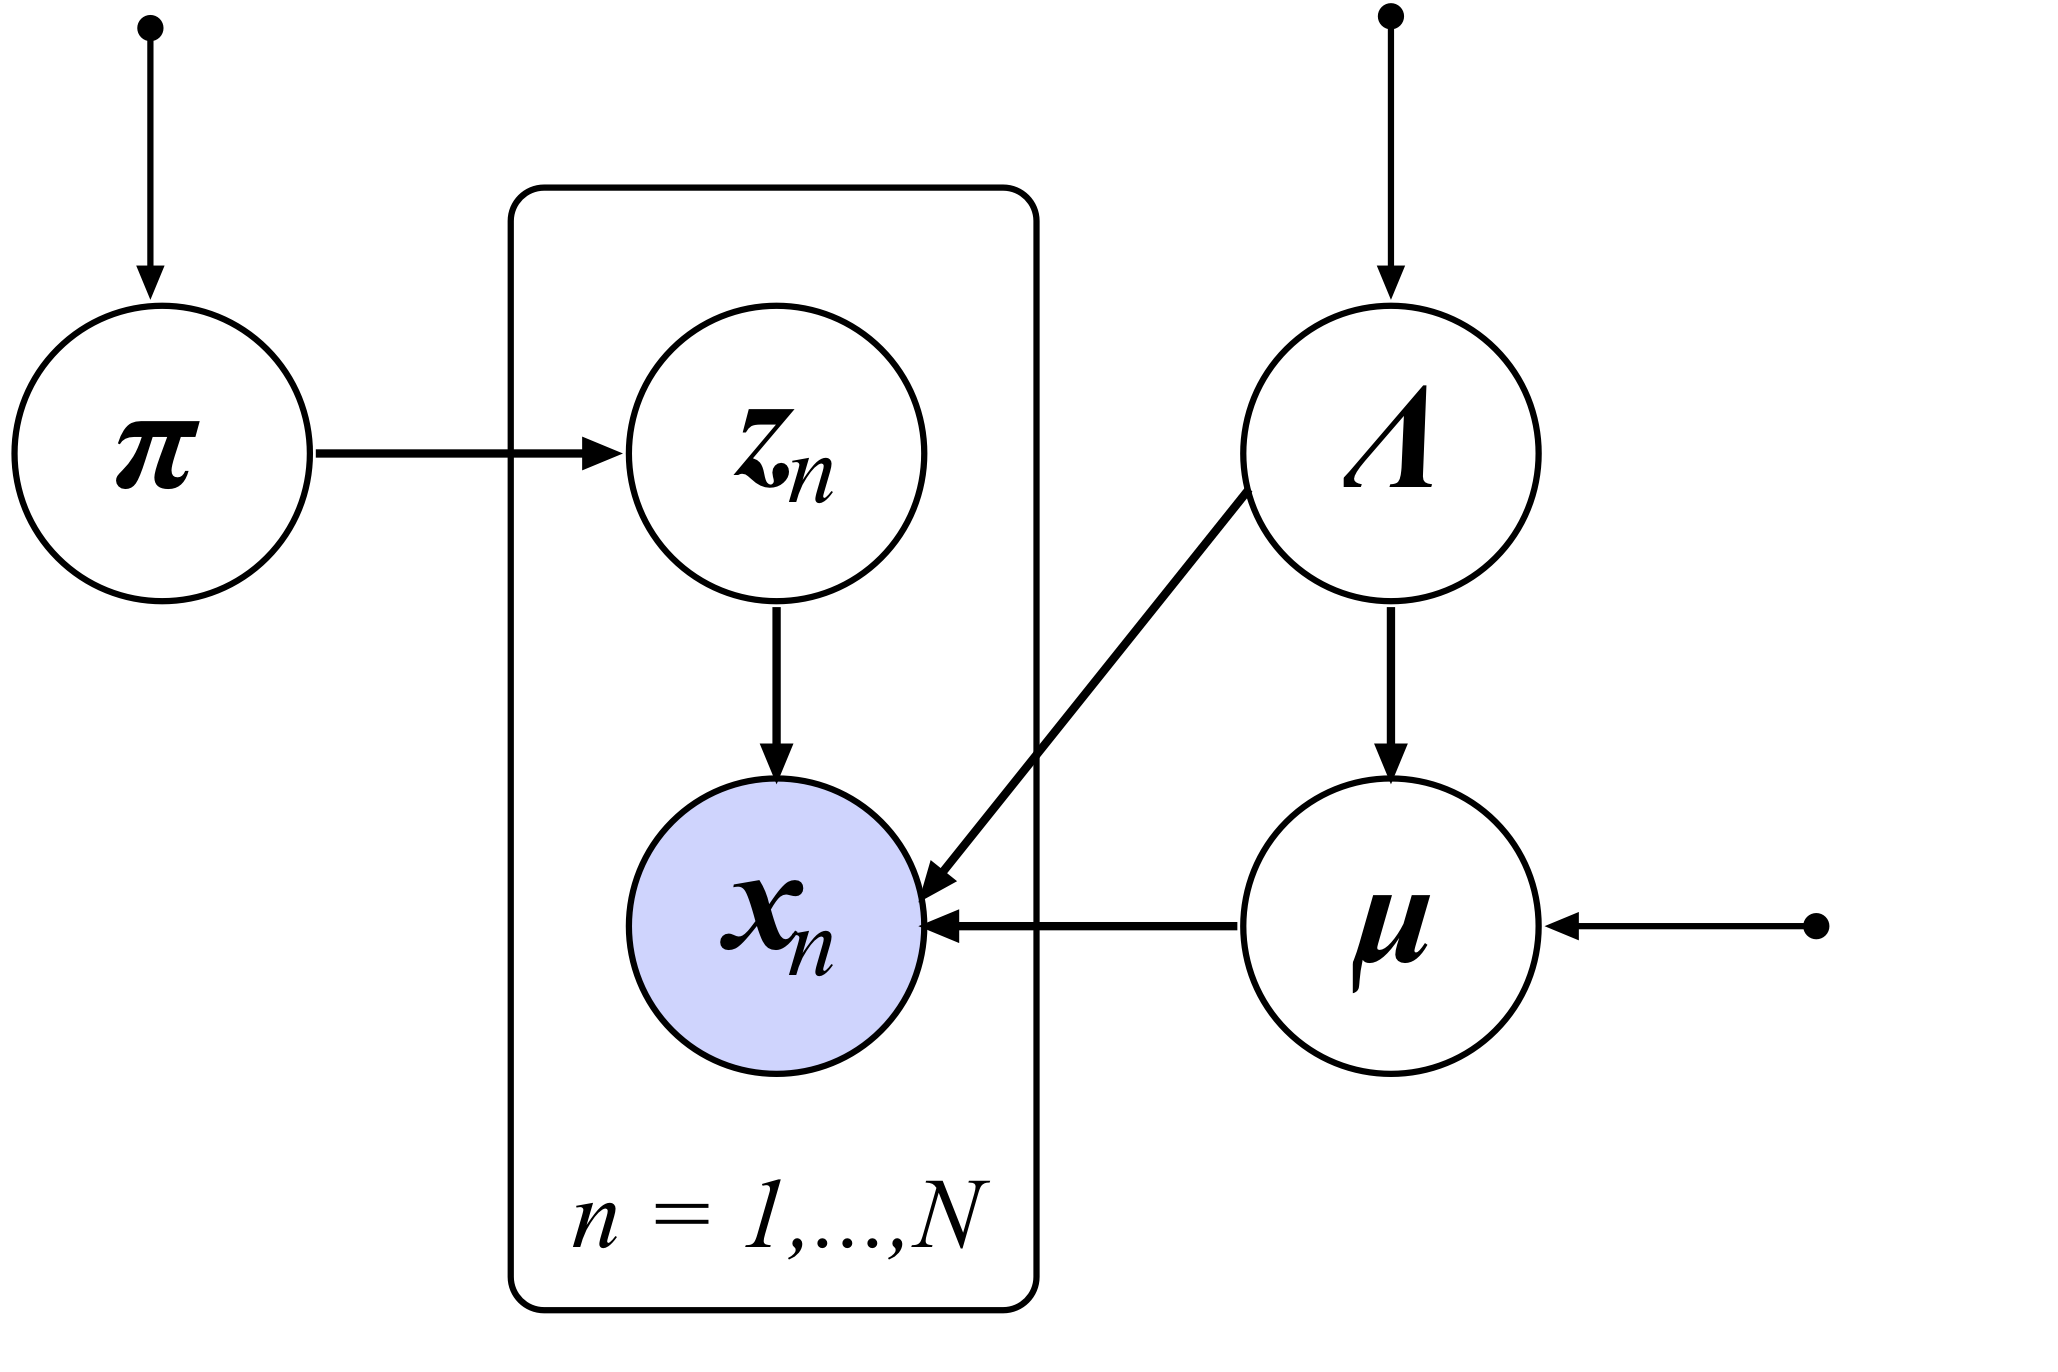
\includegraphics[width=50mm]{graph_model}
\caption{NEED TO UPDATE THIS FIGURE TO USE SIGMA INSTEAD OF GAMMA}
\end{center}
\end{figure}

\subsection{Expectation maximization}
\subsection{Simulated Annealing}

To provide a reasonable initialization for the samplers, it is useful to obtain a maximum-likelihood estimate of the model parameters. Simulated annealing is one common approach.  Our state space consists of the mean vectors and covariance matrices for each clusters, and the objective function is the negative log-likelihood of observing the data given the present parameters. We minimize the objective function to find the maximum likelihood parameters.

One important implementation decision is how to jump to a new state. For a cluster mean, we take the present estimate of the mean and add Gaussian noise distributed with a covariance matrix proportional to that of the cluster. For the cluster covariance matrix, we also add Gaussian noise with adjustable variance. However, since this noise may create an invalid covariance matrix, we must process the matrix to ensure that it remains symmetric and positive semi-definite by only modifying negative eigenvalues with some small positive epsilon and keeping the eigenvectors as unchanged as possible.

\subsubsection{Gibbs sampling}
For the Gibbs sampler, each iteration requires the following steps: 

1. Each datapoint's indicator variable $Z_n$ is drawn from a multinomial distribution with the event probabilities given by 
\begin{equation}
p(z_{nk} = 1| x_n, \mu, \Sigma, \pi)  \propto \pi_k \mathcal{N}(x_n | \mu_k, \Sigma_k)\end{equation}

2. The mixture coefficients are drawn from the conditional distribution 
\begin{equation}
p(\pi|\mathbf{Z}) = \mathrm{Dir}(\{\alpha_{0,k}+ N_k\} )
\end{equation}
where $N_k$ is the number of observations assigned to each cluster. 

3. The component means are drawn from the conditional distribution 
\begin{equation}
p(\mu_k | \Sigma_k, \mathbf{Z}, \mathbf{X}) = \mathcal{N}(\mu_k | m_k, V_k)
\end{equation}
where 
\begin{equation}
V_k^{-1} = V_0^{-1} + N_k\Sigma_k^{-1}
\end{equation}
and 
\begin{equation}
 m_k = V_k(\Sigma_k^{-1}N_k\overline{x}_k + V_0^{-1}m_0)
 \end{equation}
 with $\overline{x}_k$  defined as the mean value of the observations assigned to component $k$. 
 
 4. Finally, the component covariance matrices are drawn from the conditional distribution 
 
 \begin{equation}
 p(\Sigma_k | \mu_k, \mathbf{Z}, \mathbf{X}) = IW(\Sigma_k | S_k, \nu_0+N_k)
 \end{equation}
 where 
 \begin{equation}
S_k = S_0 + \sum_{n=1}^N z_{nk}(x_n - \mu_k)(x_n - \mu_k)^\top
\end{equation}



One common issue with using Gaussian mixture models is known as the ``label-switching problem,'' which occurs when component identities are ambiguous because the likelihood is the same if component labels are exchanged. We follow the suggestion of Gelman et al. \cite{Gelman} to resolve the ambiguity by defining $\pi_1 > \pi_2 > \pi_3$. However, this type of identifiability constraint may not always break symmetry as desired, particularly if the fractions are similar in size \cite{Stephens}. 

We use the MAP estimate obtained from expectation maximization to initialize the values of $\pi$, $\mu$, and $\Sigma$ for the Gibbs sampler. We then set $\alpha_0 = (1,1,1)$, $m_0 = (1,1,1)$, $\nu_0 = 3$ (the number of components in the mixture model), and $S_0$ and $V_0$ to the identity matrices to maintain weakly informative priors.   

\section{Results}

\subsection{Expectation maximization}
Using the Bayesian Information Criterion [insert equation here], $K = 3$ was determined to be the optimal number of components to use to model the observations in the simulated annealing and Gibbs sampling analysis. 
\subsection{Simulated annealing}
Simulated annealing requires about 1000 iterations to converge, and takes longer to run even when using a smaller sub-sample (3000 observations) of the dataset compared to EM. As a point estimate method for a Gaussian mixture model, EM appears to be more efficient. Like EM, simulated annealing finds the requests dominated by a large cluster of requests 
\begin{figure}
\begin{center}\label{SAcluster}
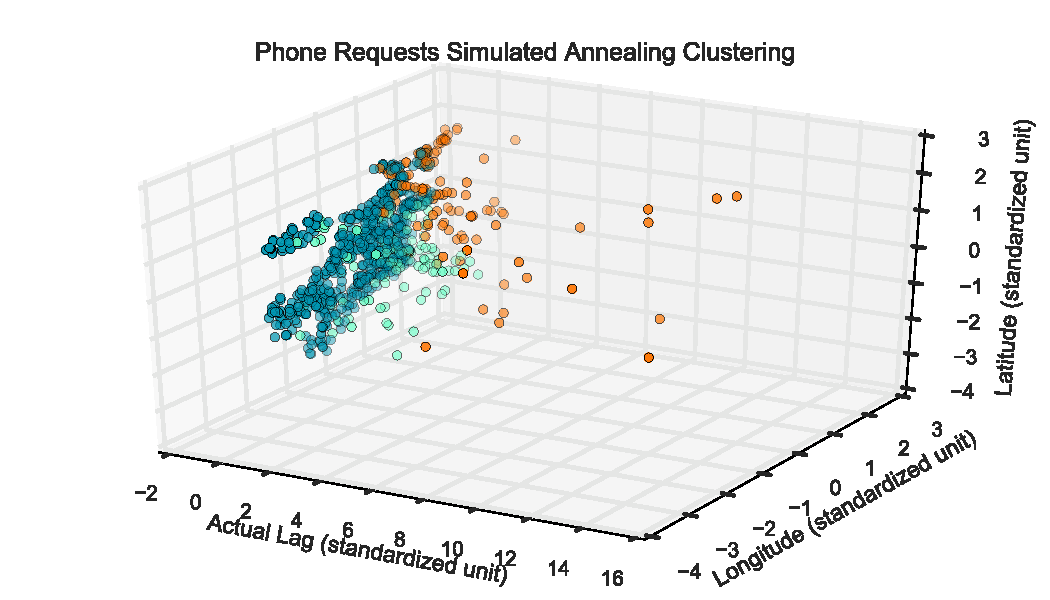
\includegraphics[width=70mm]{simulated_annealing_clustering}
\caption{Cluster assignments for call data based on simulated annealing}
\label{trace}
\end{center}
\end{figure}

\subsection{Gibbs sampling}
\begin{figure}
\begin{center}
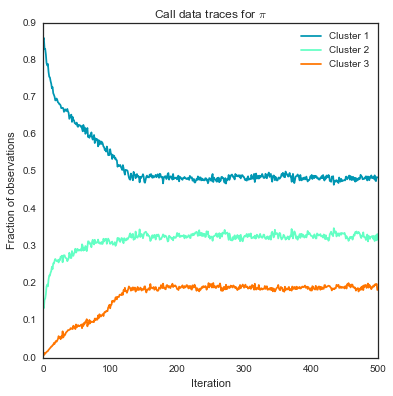
\includegraphics[width=60mm]{calldatapitrace}
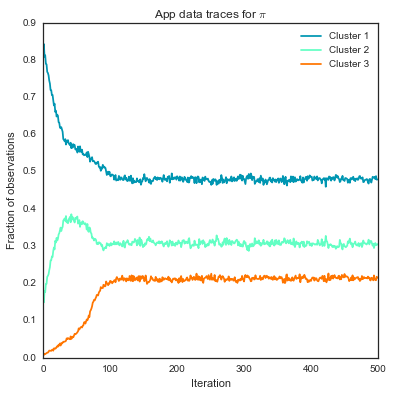
\includegraphics[width=60mm]{appdatapitrace}
\caption{Gibbs sampler traces for the $\pi$ parameter}
\label{trace}
\end{center}
\end{figure}

The Gibbs sampler was run for a total of 500 iterations for both the constituent call and app data. Inspection of the trace plots suggest that convergence is achieved after 150 iterations (see Fig. \ref{trace} for sample trace plots), so a burn-in of 150 iterations is applied for calculation of the posterior means and uncertainties, listed in Table \ref{comparison}.
DISCUSSION/COMPARISON OF RESULTS


\begin{table*}[h]
\caption{Gibbs results}
\label{comparison}
\begin{center}
\begin{tabular}{c|c|c}
%\multicolumn{1}{c}{\bf PART}  &\multicolumn{1}{c}{\bf DESCRIPTION} \\
Parameter & Constituent Call & App data\\
\hline
$\pi$ &
$\left(\begin{array}{ccc} .484\pm.006 & .328\pm.006  &.189\pm.005 \end{array}\right)$ 

\\

$\mu_1 $ &       
$\left(\begin{array}{ccc} -.419\pm.001 & -.13\pm.02  &-.11\pm.02 \end{array}\right)$ 
     
&\\
\\
$\Sigma_1$ & 
$\left(\begin{array}{ccc} .0018 & -.0063  &-.0065 \\
-.0063 & 1.1 &.60 \\
-.0065 & .60 & 1.1
\end{array}\right)$ 

& 

\\
$\mu_2 $           &  \\
$\Sigma_2$  & \\
$\mu_3$ & \\
$\Sigma_3$ &  \\
\end{tabular}
\caption*{Variables listed in order of (response time, longitude, latitude) in standardized units. The mean response time is 13.2 days with standard deviation 29.1 days. The mean latitude is 42.326 with standard deviation 0.034. The mean longitude is -71.083 with standard deviation 0.035. }
\end{center}
\end{table*}
\subsection{Posterior predictive}
To assess how well the model describes the data, we simulate data with the posterior predictive distribution. The posterior predictive distribution is generated by sampling from the posterior distribution obtained through Gibbs sampling, then using those parameter values to sample from the likelihood. 

%\begin{table*}[h]
%\caption{Method comparisons}
%\label{comparison}
%\begin{center}
%\begin{tabular}{c|c|c|c|c}
%%\multicolumn{1}{c}{\bf PART}  &\multicolumn{1}{c}{\bf DESCRIPTION} \\
%Parameter & Simulated Annealing & EM MLE & EM MAP & Gibbs \\
%\hline
%$\pi$ & \\
%$\mu_1 $             &\\
%$\Sigma_1$ & 
%$\left(\begin{array}{ccc} .0018 & -.0063  &-.0065 \\
%-.0063 & 1.1 &0.60 \\
%-.0065 & 0.60 & 1.1
%\end{array}\right)$ & 
%$\left(\begin{array}{ccc} .0018 & -.0063  &-.0065 \\
%-.0063 & 1.1 &0.60 \\
%-.0065 & 0.60 & 1.1
%\end{array}\right)$ & 
%$\left(\begin{array}{ccc} .0018 & -.0063  &-.0065 \\
%-.0063 & 1.1 &0.60 \\
%-.0065 & 0.60 & 1.1
%\end{array}\right)$ 
%& 
%
%$\left(\begin{array}{ccc} .0018 & -.0063  &-.0065 \\
%-.0063 & 1.1 &0.60 \\
%-.0065 & 0.60 & 1.1
%\end{array}\right)$ 
%
%\\
%$\mu_2 $           &  \\
%$\Sigma_2$  & \\
%$\mu_3$ & \\
%$\Sigma_3$ &  \\
%\end{tabular}
%\caption*{Variables are listed in order of (response time, longitude, latitude) in standardized units. The mean response time is 13.2 days with standard deviation 29.1 days. The mean latitude is 42.326 with standard deviation 0.034. The mean longitude is -71.083 with standard deviation 0.035. }
%\end{center}
%\end{table*}
\subsection{Comparing results from different methods}

\section{Conclusion}



\bibliographystyle{abbrv}
\bibliography{GMMBib}

\end{document}





